\scanpage{20}
\mspage{\textcircled{3}}

\textbf{ACADEMIE D'AIX-MARSEILLE}\\
\rule{3cm}{.4pt}\\
\textbf{INSPECTION ACADEMIQUE}\\
\textbf{DE VAUCLUSE}\\
\rule{1cm}{.4pt}

\diagram{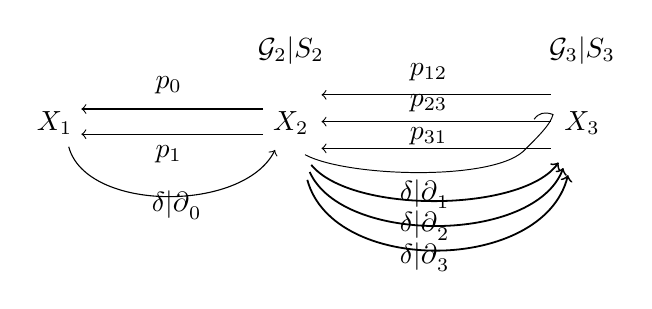
\begin{tikzpicture}[x=1cm,y=1cm]
\node at (0,0) {$X_1$}; \node at (3,0) {$X_2$}; \node at (6.7,0) {$X_3$};
\node at (3,.92) {$\unsure{\mathcal G_2|\mathfrak S_2}$};
\node at (6.7,.92) {$\unsure{\mathcal G_3|\mathfrak S_3}$};
\draw[->] (2.65,.18)--(.34,.18); \node at (1.45,.48) {$p_0$};
\draw[->] (2.65,-.14)--(.34,-.14); \node at (1.45,-.39) {$p_1$};
\draw[->] (.18,-.30)..controls(.40,-1.13)and(2.40,-1.14)..(2.80,-.34);
\node at (1.55,-1.04) {$\unsure{\delta|\partial}_0$};
\draw[->] (6.30,.36)--(3.39,.36); \node at (4.75,.65) {$p_{12}$};
\draw[->] (6.30,.02)--(3.39,.02); \node at (4.75,.25) {$p_{23}$};
\draw[->] (6.30,-.32)--(3.39,-.32); \node at (4.75,-.16) {$p_{31}$};
\draw[line width=.35pt] (3.18,-.40)..controls(3.70,-.68)and(5.52,-.74)..(5.95,-.36)
 ..controls(6.12,-.19)and(6.30,-.02)..(6.33,.11)
 ..controls(6.22,.15)and(6.15,.13)..(6.09,.05);
\draw[->,line width=.65pt] (3.26,-.53)..controls(3.78,-1.16)and(5.95,-1.13)..(6.40,-.50);
\draw[->,line width=.65pt] (3.24,-.62)..controls(3.66,-1.55)and(6.10,-1.53)..(6.46,-.57);
\draw[->,line width=.65pt] (3.21,-.72)..controls(3.54,-1.94)and(6.21,-1.91)..(6.52,-.66);
\node at (4.70,-.90) {$\unsure{\delta|\partial}_1$};
\node at (4.70,-1.30) {$\unsure{\delta|\partial}_2$};
\node at (4.70,-1.70) {$\unsure{\delta|\partial}_3$};
\end{tikzpicture}}
\margin{$\rho,\sigma_1,\sigma_2,\sigma_3$}

\deleted{$\unsure{p|\rho}=\unsure{q|\sigma}$}

\figure{\begin{tikzpicture}[x=1cm,y=1cm]
\node at (-1.8,.45) {$X_2$}; \node at (2.2,.45) {$X_1\times X_1$};
\node at (2.2,-1.10) {$X_1$};
\node at (-2.95,.45) {$\unsure{\mathcal G_2|\mathfrak S_2}$};
\draw[->] (-1.40,.45)--(1.44,.45); \draw(1.23,.57)--(1.40,.45)--(1.23,.33);
\node at (.10,.83) {$(p_0,p_1)\ \text{épi}$};
\node at (.16,1.50) {$p_0\sigma$}; \node at (.16,1.18) {$\Vert$};
\draw[->] (2.20,-.75)--(2.20,.10);
\draw(2.20,-.75)..controls(2.37,-.81)and(2.42,-.69)..(2.39,-.60);
\draw[->] (1.83,-.92)--(-1.45,.19);
\node at (.12,-.72) {$\unsure{\delta|\partial}_0$};
\draw(-2.23,1.70)--(2.55,1.85)..controls(2.95,1.83)and(2.96,1.76)..(2.96,1.33);
\draw(2.97,1.10)--(3.10,-1.28)..controls(3.10,-1.54)and(2.82,-1.57)..(-2.23,-1.55);
\draw(-2.23,-1.55)--(-2.23,1.15);
\node at (-2.10,-2.52) {iso ???}; \draw(-2.10,-2.52) ellipse (1.05 and .49);
\draw[->] (-.32,.19)..controls(-.71,-.92)and(-3.26,-1.92)..(-2.91,-2.40);
\end{tikzpicture}}

\diagram{\begin{tikzpicture}[x=1cm,y=1cm]
\node at (0,0) {$X_3$}; \node at (3.55,0) {$X_2\times X_1$};
\node at (7.80,0) {$X_1\times X_1\times X_1$};
\draw[->] (.35,0)--(2.77,0); \draw(2.55,.12)--(2.72,0)--(2.55,-.12);
\node at (1.55,.35) {$(p_{12},q_3)\ \text{épi}$};
\draw[->] (4.32,0)--(6.48,0); \draw(6.25,.12)--(6.42,0)--(6.25,-.12);
\node at (5.43,.36) {$(p_0,p_1)\times\mathrm{id}_{X_1}$};
\draw[line width=.45pt] (-.27,.88)--(1.63,.83)..controls(2.25,.81)and(2.58,.53)..(3.04,.53)
 --(5.80,.53)..controls(5.96,.53)and(6.04,.58)..(6.06,.68);
\end{tikzpicture}}

\diagram{\begin{tikzpicture}[x=1cm,y=1cm]
\node at (0,0) {$X_3$};
\node at (3.72,0) {$\overset{(p_1)}{X_2}\times_{X_1}\overset{(p_0)}{X_2}$};
\node at (8.12,0) {$X_2\times_{X_1}(X_1\times X_1)$};
\draw[->] (.35,0)--(2.52,0); \draw(2.30,.12)--(2.47,0)--(2.30,-.12);
\node at (1.43,.34) {épi}; \node at (1.43,-.39) {$(p_{12},p_{23})$};
\draw[->] (4.93,0)--(6.22,0); \draw(6.00,.12)--(6.17,0)--(6.00,-.12);
\node at (5.58,.35) {épi};
\draw(-.47,.66)--(4.99,.73);
\draw(5.12,.60)--(5.15,-.54);
\draw(4.99,-.67)--(-.43,-.63);
\draw(-.55,-.51)--(-.57,.55);
\end{tikzpicture}}

\diagram{\begin{tikzcd}[ampersand replacement=\&]
\mathbb E_1\arrow[r]\arrow[d]\&\mathbb E_2\arrow[d]\\
\mathbb E_2\arrow[r]\&\mathbb E_3
\end{tikzcd}}

\figure{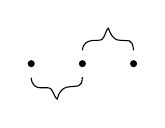
\begin{tikzpicture}[x=1cm,y=1cm]
\fill(0,0)circle(.045); \fill(.65,0)circle(.045); \fill(1.30,0)circle(.045);
\draw(0,-.18)..controls(.02,-.38)and(.20,-.27)..(.25,-.32)
 ..controls(.28,-.35)and(.30,-.44)..(.33,-.45)
 ..controls(.35,-.36)and(.40,-.31)..(.45,-.30)
 ..controls(.60,-.27)and(.64,-.32)..(.65,-.17);
\draw(.65,.17)..controls(.67,.35)and(.86,.27)..(.90,.31)
 ..controls(.94,.34)and(.95,.44)..(.98,.45)
 ..controls(1.01,.36)and(1.05,.31)..(1.10,.30)
 ..controls(1.25,.28)and(1.28,.33)..(1.30,.17);
\end{tikzpicture}}

\diagram{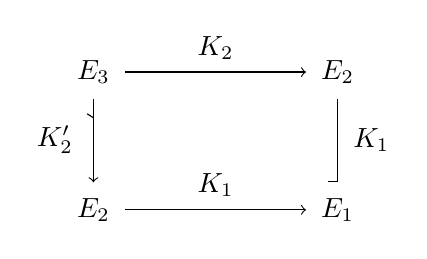
\begin{tikzpicture}[x=1cm,y=1cm]
\node at (0,0) {$\mathbb E_3$}; \node at (3.1,0) {$\mathbb E_2$};
\node at (0,-1.75) {$\mathbb E_2$}; \node at (3.1,-1.75) {$\mathbb E_1$};
\draw[->] (.40,0)--(2.70,0); \node at (1.55,.30) {$K_2$};
\draw[->] (0,-.34)--(0,-1.40); \draw(0,-.58)--(-.08,-.53);
\node at (-.49,-.86) {$K'_2$};
\draw(3.10,-.34)--(3.10,-1.39)--(2.98,-1.39);
\node at (3.53,-.86) {$K_1$};
\draw[->] (.40,-1.75)--(2.70,-1.75); \node at (1.55,-1.43) {$K_1$};
\end{tikzpicture}}

\figure{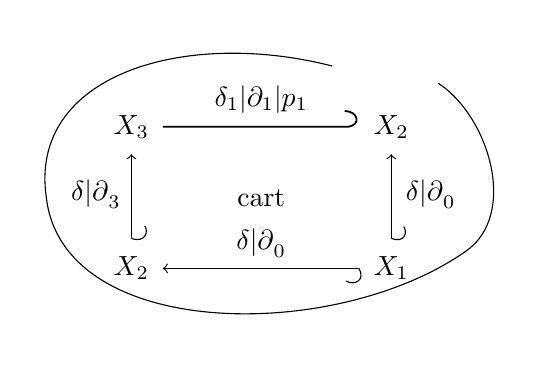
\begin{tikzpicture}[x=1cm,y=1cm]
\node at (0,0) {$X_3$}; \node at (3.3,0) {$X_2$};
\node at (0,-1.80) {$X_{\unsure{2}}$}; \node at (3.3,-1.80) {$X_1$};
\draw[line width=.65pt] (.40,0)--(2.76,0)..controls(2.91,.02)and(2.89,.19)..(2.71,.20);
\node at (1.65,.34) {$\unsure{\delta_1|\partial_1|p_1}$};
\draw[->] (0,-1.42)--(0,-.35);
\draw(0,-1.42)..controls(.18,-1.48)and(.22,-1.33)..(.17,-1.26);
\node at (-.45,-.86) {$\unsure{\delta|\partial}_3$};
\draw[->] (3.30,-1.42)--(3.30,-.35);
\draw(3.30,-1.42)..controls(3.47,-1.48)and(3.51,-1.35)..(3.46,-1.27);
\node at (3.80,-.86) {$\unsure{\delta|\partial}_0$};
\draw[->] (2.89,-1.80)--(.40,-1.80);
\draw(2.89,-1.80)..controls(2.98,-1.96)and(2.82,-2.02)..(2.73,-1.96);
\node at (1.65,-1.48) {$\unsure{\delta|\partial}_0$};
\node at (1.65,-.91) {cart};
\draw(2.55,.77)..controls(.68,1.25)and(-1.31,.66)..(-1.08,-.90)
 ..controls(-.87,-2.72)and(2.59,-2.75)..(4.25,-1.58)
 ..controls(4.91,-1.12)and(4.55,.12)..(3.90,.55);
\end{tikzpicture}}

\diagram{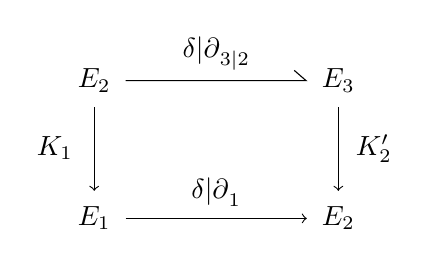
\begin{tikzpicture}[x=1cm,y=1cm]
\node at (0,0) {$\mathbb E_2$}; \node at (3.1,0) {$\mathbb E_3$};
\node at (0,-1.75) {$\mathbb E_1$}; \node at (3.1,-1.75) {$\mathbb E_2$};
\draw(.40,0)--(2.69,0)--(2.54,.13);
\node at (1.55,.34) {$\unsure{\delta|\partial}_{\unsure{3|2}}$};
\draw[->] (0,-.34)--(0,-1.40); \node at (-.50,-.86) {$K_{\unsure{1}}$};
\draw[->] (3.10,-.34)--(3.10,-1.40); \node at (3.55,-.86) {$K'_2$};
\draw[->] (.40,-1.75)--(2.70,-1.75);
\node at (1.55,-1.42) {$\unsure{\delta|\partial}_1$};
\end{tikzpicture}}

\figure{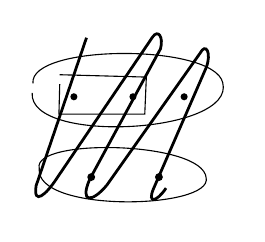
\begin{tikzpicture}[x=1cm,y=1cm]
\draw(-1.17,.17)..controls(-1.22,.67)and(1.12,.68)..(1.24,.18)
 ..controls(1.41,-.47)and(-1.23,-.61)..(-1.18,.05);
\draw(-.83,.28)--(.27,.25)--(.25,-.22)--(-.84,-.22)--(-.83,.16);
\fill(-.65,0)circle(.045); \fill(.10,0)circle(.045); \fill(.75,0)circle(.045);
\draw(-1.09,-.91)..controls(-1.19,-.52)and(.99,-.56)..(1.03,-1.03)
 ..controls(1.11,-1.43)and(-1.15,-1.48)..(-1.09,-.91);
\fill(-.43,-1.02)circle(.05); \fill(.43,-1.02)circle(.05);
\draw[line width=1pt] (-.49,.75)--(-1.13,-1.13)
 ..controls(-1.17,-1.39)and(-1.00,-1.24)..(-.87,-1.04)
 --(.35,.76)..controls(.42,.86)and(.49,.76)..(.45,.61)
 --(-.45,-1.05)..controls(-.58,-1.35)and(-.42,-1.35)..(-.23,-1.12)
 --(.95,.55)..controls(1.03,.70)and(1.10,.55)..(1.03,.37)
 --(.36,-1.17)..controls(.28,-1.36)and(.40,-1.34)..(.52,-1.16);
\end{tikzpicture}}

\figure{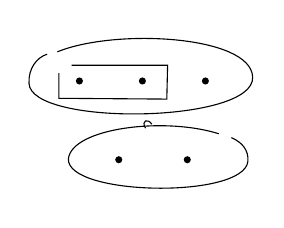
\begin{tikzpicture}[x=1cm,y=1cm]
\draw(-.93,.37)..controls(-.20,.67)and(1.53,.58)..(1.55,.05)
 ..controls(1.58,-.54)and(-1.27,-.58)..(-1.29,-.03)
 ..controls(-1.30,.16)and(-1.19,.30)..(-1.06,.34);
\draw(-.75,.20)--(.47,.20)--(.46,-.23)--(-.91,-.22)--(-.91,.10);
\fill(-.65,0)circle(.045); \fill(.15,0)circle(.045); \fill(.95,0)circle(.045);
\draw(1.12,-.67)..controls(.42,-.45)and(-.75,-.60)..(-.79,-.99)
 ..controls(-.81,-1.46)and(1.44,-1.50)..(1.49,-1.02)
 ..controls(1.50,-.88)and(1.42,-.78)..(1.28,-.72);
\draw(.19,-.60)..controls(.13,-.50)and(.22,-.47)..(.27,-.55);
\fill(-.15,-1.00)circle(.045); \fill(.72,-1.00)circle(.045);
\end{tikzpicture}}

\figure{\unsure{\deleted{\mbox{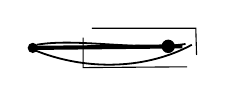
\begin{tikzpicture}[x=1cm,y=1cm]
\draw[line width=1.5pt] (-.80,0)--(1.12,.02);
\fill(-.78,0)circle(.065); \fill(.94,.02)circle(.085);
\draw(-.03,.25)--(1.29,.25)--(1.30,-.09);
\draw(1.18,-.24)--(-.14,-.25)--(-.14,.13);
\draw[line width=.65pt] (-.78,-.02)..controls(-.08,-.31)and(.69,-.26)..(1.24,.04);
\draw[line width=.65pt] (-.73,.04)..controls(-.22,.13)and(.57,-.04)..(1.16,.05);
\end{tikzpicture}}}}}

\figure{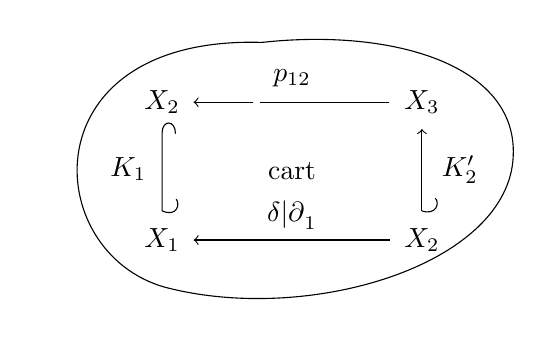
\begin{tikzpicture}[x=1cm,y=1cm]
\node at (0,0) {$X_2$}; \node at (3.3,0) {$X_3$};
\node at (0,-1.75) {$X_1$}; \node at (3.3,-1.75) {$X_2$};
\draw[<-] (.40,0)--(1.15,0); \draw(1.24,0)--(2.88,0);
\node at (1.65,.31) {$p_{12}$};
\draw(0,-1.38)--(0,-.39)..controls(0,-.22)and(.17,-.22)..(.17,-.40);
\draw(0,-1.38)..controls(.19,-1.46)and(.23,-1.30)..(.18,-1.23);
\node at (-.43,-.85) {$K_1$};
\draw[->] (3.30,-1.38)--(3.30,-.34);
\draw(3.30,-1.38)..controls(3.48,-1.44)and(3.53,-1.28)..(3.47,-1.22);
\node at (3.78,-.85) {$K'_2$};
\draw[->] (2.89,-1.75)--(.40,-1.75);
\node at (1.65,-1.43) {$\unsure{\delta|\partial}_1$};
\node at (1.65,-.87) {cart};
\draw(1.27,.76)..controls(-1.70,.85)and(-1.55,-1.91)..(.04,-2.35)
 ..controls(1.87,-2.83)and(4.42,-2.06)..(4.46,-.67)
 ..controls(4.50,.49)and(2.90,.94)..(1.27,.76);
\end{tikzpicture}}

\diagram{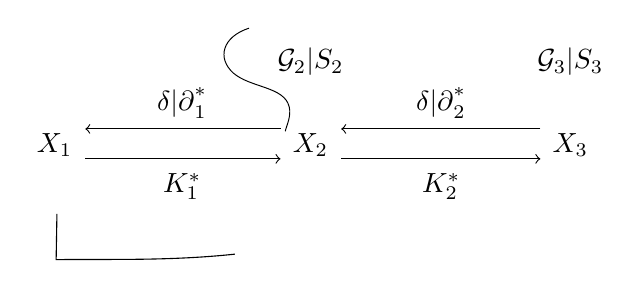
\begin{tikzpicture}[x=1cm,y=1cm]
\node at (0,0) {$X_1$}; \node at (3.25,0) {$X_2$}; \node at (6.55,0) {$X_3$};
\node at (3.25,1.05) {$\unsure{\mathcal G_2|\mathfrak S_2}$};
\node at (6.55,1.05) {$\unsure{\mathcal G_3|\mathfrak S_3}$};
\draw[->] (2.87,.20)--(.39,.20);
\node at (1.62,.53) {${\unsure{\delta|\partial}}_1^*$};
\draw[->] (.39,-.18)--(2.87,-.18); \node at (1.62,-.53) {$K_{\unsure{1}}^*$};
\draw[->] (6.17,.20)--(3.64,.20);
\node at (4.91,.53) {${\unsure{\delta|\partial}}_2^*$};
\draw[->] (3.64,-.18)--(6.17,-.18); \node at (4.91,-.53) {$K_2^*$};
\draw[line width=.35pt] (2.47,1.48)..controls(2.13,1.37)and(2.06,1.10)..(2.27,.91)
 ..controls(2.49,.72)and(2.92,.74)..(2.98,.48)
 ..controls(3.01,.36)and(2.94,.23)..(2.93,.17);
\draw(.03,-.88)--(.02,-1.46)..controls(.65,-1.45)and(1.45,-1.48)..(2.29,-1.39);
\end{tikzpicture}}

\deleted{$\unsure{\mathbb E}$}

\noindent Supposons $X_1$ réduit\\
à un élément, donc\\
$X_2$ est un $\unsure{\mathcal G_2|\mathfrak S_2}$-ens. à pt\\
fixe marqué $\unsure{\delta|\partial}_2$, $X_3$ un\\
$\unsure{\mathcal G_3|\mathfrak S_3}$-ens. à pt fixe marqué $\unsure{\delta|\partial}_3$

\diagram{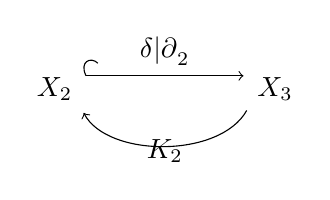
\begin{tikzpicture}[x=1cm,y=1cm]
\node at (0,0) {$X_2$}; \node at (2.8,0) {$X_3$};
\draw[->] (.40,.17)--(2.40,.17);
\draw(.40,.17)..controls(.31,.35)and(.46,.42)..(.55,.33);
\node at (1.40,.48) {$\unsure{\delta|\partial}_2$};
\draw[->] (2.44,-.27)..controls(2.10,-.88)and(.67,-.87)..(.37,-.30);
\node at (1.40,-.78) {$K_2$};
\end{tikzpicture}}

\deleted{$\unsure{\delta|\partial}_{\unsure{2}}$} $\unsure{\delta|\partial}_2$ et $K_2$\\
compatibles avec\\
les \deleted{\unsure{pts fixes}} \inserted{\unsure{ponctuations|pointations|structures}}\\
par $\unsure{\delta|\partial}_2,\unsure{\delta|\partial}_3$, avec
\[
K_2\unsure{\delta|\partial}_2=\mathrm{id}_{X_2}
\]

\diagram{\begin{tikzcd}[ampersand replacement=\&]
\mathbb E_1\arrow[r,hook]\&\mathbb E_2\arrow[l,bend left=45]
\end{tikzcd}}

\figure{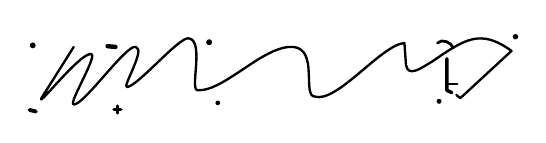
\begin{tikzpicture}[x=1cm,y=1cm,line cap=round,line join=round]
\draw[line width=.85pt] (.57,.75)--(.16,.10)
 ..controls(.10,-.03)and(.63,.65)..(.78,.66)
 ..controls(.91,.69)and(.49,.02)..(.57,.02)
 ..controls(.69,.00)and(1.25,.80)..(1.36,.75)
 ..controls(1.49,.72)and(1.17,.22)..(1.25,.24)
 ..controls(1.40,.27)and(1.91,.88)..(2.03,.86)
 ..controls(2.24,.83)and(2.03,.18)..(2.15,.20)
 ..controls(2.49,.19)and(2.99,.78)..(3.36,.75)
 ..controls(3.68,.72)and(3.47,.13)..(3.63,.12)
 ..controls(3.91,.03)and(4.48,.78)..(4.77,.80)
 --(4.79,.52)..controls(4.82,.36)and(4.98,.48)..(5.13,.57)
 ..controls(5.55,.86)and(5.74,.98)..(6.13,.70)
 --(5.48,.10)--(5.43,.14);
\fill(.05,.77)circle(.037); \draw[line width=1.4pt] (.01,-.05)--(.09,-.07);
\draw[line width=1.6pt] (1.00,.76)--(1.10,.75);
\draw[line width=1.15pt] (1.13,.00)--(1.13,-.09); \draw[line width=1.15pt] (1.08,-.04)--(1.17,-.04);
\fill(2.29,.81)circle(.038); \fill(2.40,.04)circle(.030);
\draw[line width=1pt] (5.19,.80)..controls(5.25,.86)and(5.36,.81)..(5.39,.74);
\fill(6.18,.88)circle(.035); \fill(5.21,.06)circle(.032);
\draw[line width=1.3pt] (5.31,.60)--(5.31,.20)--(5.37,.17);
\draw[line width=.9pt] (5.30,.28)--(5.44,.28);
\end{tikzpicture}}

\margin{19}
